\documentclass[conference]{IEEEtran}
\usepackage{cite}
\usepackage{amsmath,amssymb,amsfonts}
\usepackage{graphicx}
\usepackage{textcomp}
\usepackage{xcolor}
\usepackage{url}
\usepackage{booktabs}

\begin{document}

\title{Task [A1]: [Breast Cancer Diagnosis from Cell-Nucleus Measurements]}

\author{\IEEEauthorblockN{Muhammad Zaryab Attiq}
\IEEEauthorblockA{Roll No. 70176119 \quad Section A\\
Repository: \url{https://github.com/Vex456/AI101-ML-Assignment-70176119}\\
Instructor: Dr. Muhammad Awais, AI Architect}
}

\maketitle

\section{Introduction}
Breast cancer is among the most prevalent life-threatening malignancies globally. Automated morphological analysis of fine-needle aspirate (FNA) cell nuclei offers an objective, non-invasive diagnostic pathway. In this work, we formulate an asymmetric supervised classification framework on the Wisconsin Diagnostic Breast Cancer (WDBC) dataset comprising 569 patients and 30 nuclear descriptors. Because a missed malignancy (false negative) carries lethal clinical consequences compared to a false positive, we train, tune, and compare four supervised paradigms—Logistic Regression, Support Vector Machines (RBF), Random Forest, and Gradient Boosted Decision Trees (GBDT)—embedded in zero-leakage scikit-learn pipelines. By calibrating the decision threshold, our champion model elevates malignant recall to 95.24\% with an ROC-AUC of 0.9947, demonstrating how threshold engineering aligns statistical machine learning with clinical screening safety.

\section{Problem Statement}
Given an input vector $\mathbf{x} \in \mathbb{R}^{30}$ capturing ten nuclear morphometric properties across mean, standard error, and extreme (worst) values, the task is to learn a decision classifier $f: \mathbf{x} \mapsto y \in \{0, 1\}$, where $y=1$ denotes a malignant tumor (positive class) and $y=0$ denotes a benign condition. In clinical screening, false negatives incur an order of magnitude higher penalty than false positives. Consequently, standard accuracy is uninformative. The formal learning objective is to maximize positive-class Recall $\frac{\text{TP}}{\text{TP} + \text{FN}}$ and ROC-AUC subject to the operational constraint $\text{Recall}(\tau) \ge 0.95$ under a calibrated decision threshold $\tau$.

\section{Dataset Used}
We employ the Breast Cancer Wisconsin (Diagnostic) dataset from the UCI Machine Learning Repository (ID: 17)~\cite{street1993}. The corpus contains 569 patient samples with zero missing values, consisting of 212 malignant cases (37.26\%) and 357 benign cases (62.74\%). The 30 features quantify nuclear geometric attributes extracted from digitized microscopic images: radius, texture, perimeter, area, smoothness, compactness, concavity, concave points, symmetry, and fractal dimension.

\section{Dataset Statistics}
Table~\ref{tab:dataset_stats} outlines the corpus partition and descriptive metrics. Intense geometric collinearity is observed among size parameters: \texttt{mean radius}, \texttt{mean perimeter}, and \texttt{mean area} exhibit pairwise correlations $r > 0.98$. Malignant nuclei display substantially elevated mean area (978.3 vs. 462.8 $\mu\text{m}^2$) and mean concavity (0.160 vs. 0.046) compared to benign counterparts.

\begin{table}[htbp]
\caption{Dataset statistics and clinical distribution.}
\label{tab:dataset_stats}
\centering
\begin{tabular}{lr}
\toprule
\textbf{Property} & \textbf{Value} \\
\midrule
Total patient samples & 569 \\
Morphological continuous features & 30 \\
Missing values & 0 (0.0\%) \\
Class balance & 212 Malignant (37.26\%) / 357 Benign (62.74\%) \\
Train / test split ratio & 455 (80.0\%) / 114 (20.0\%) \\
Positive class (Malignant) in test split & 42 samples (36.84\%) \\
Feature normalization & StandardScaler inside Pipeline \\
\bottomrule
\end{tabular}
\end{table}

\begin{figure}[htbp]
\centering
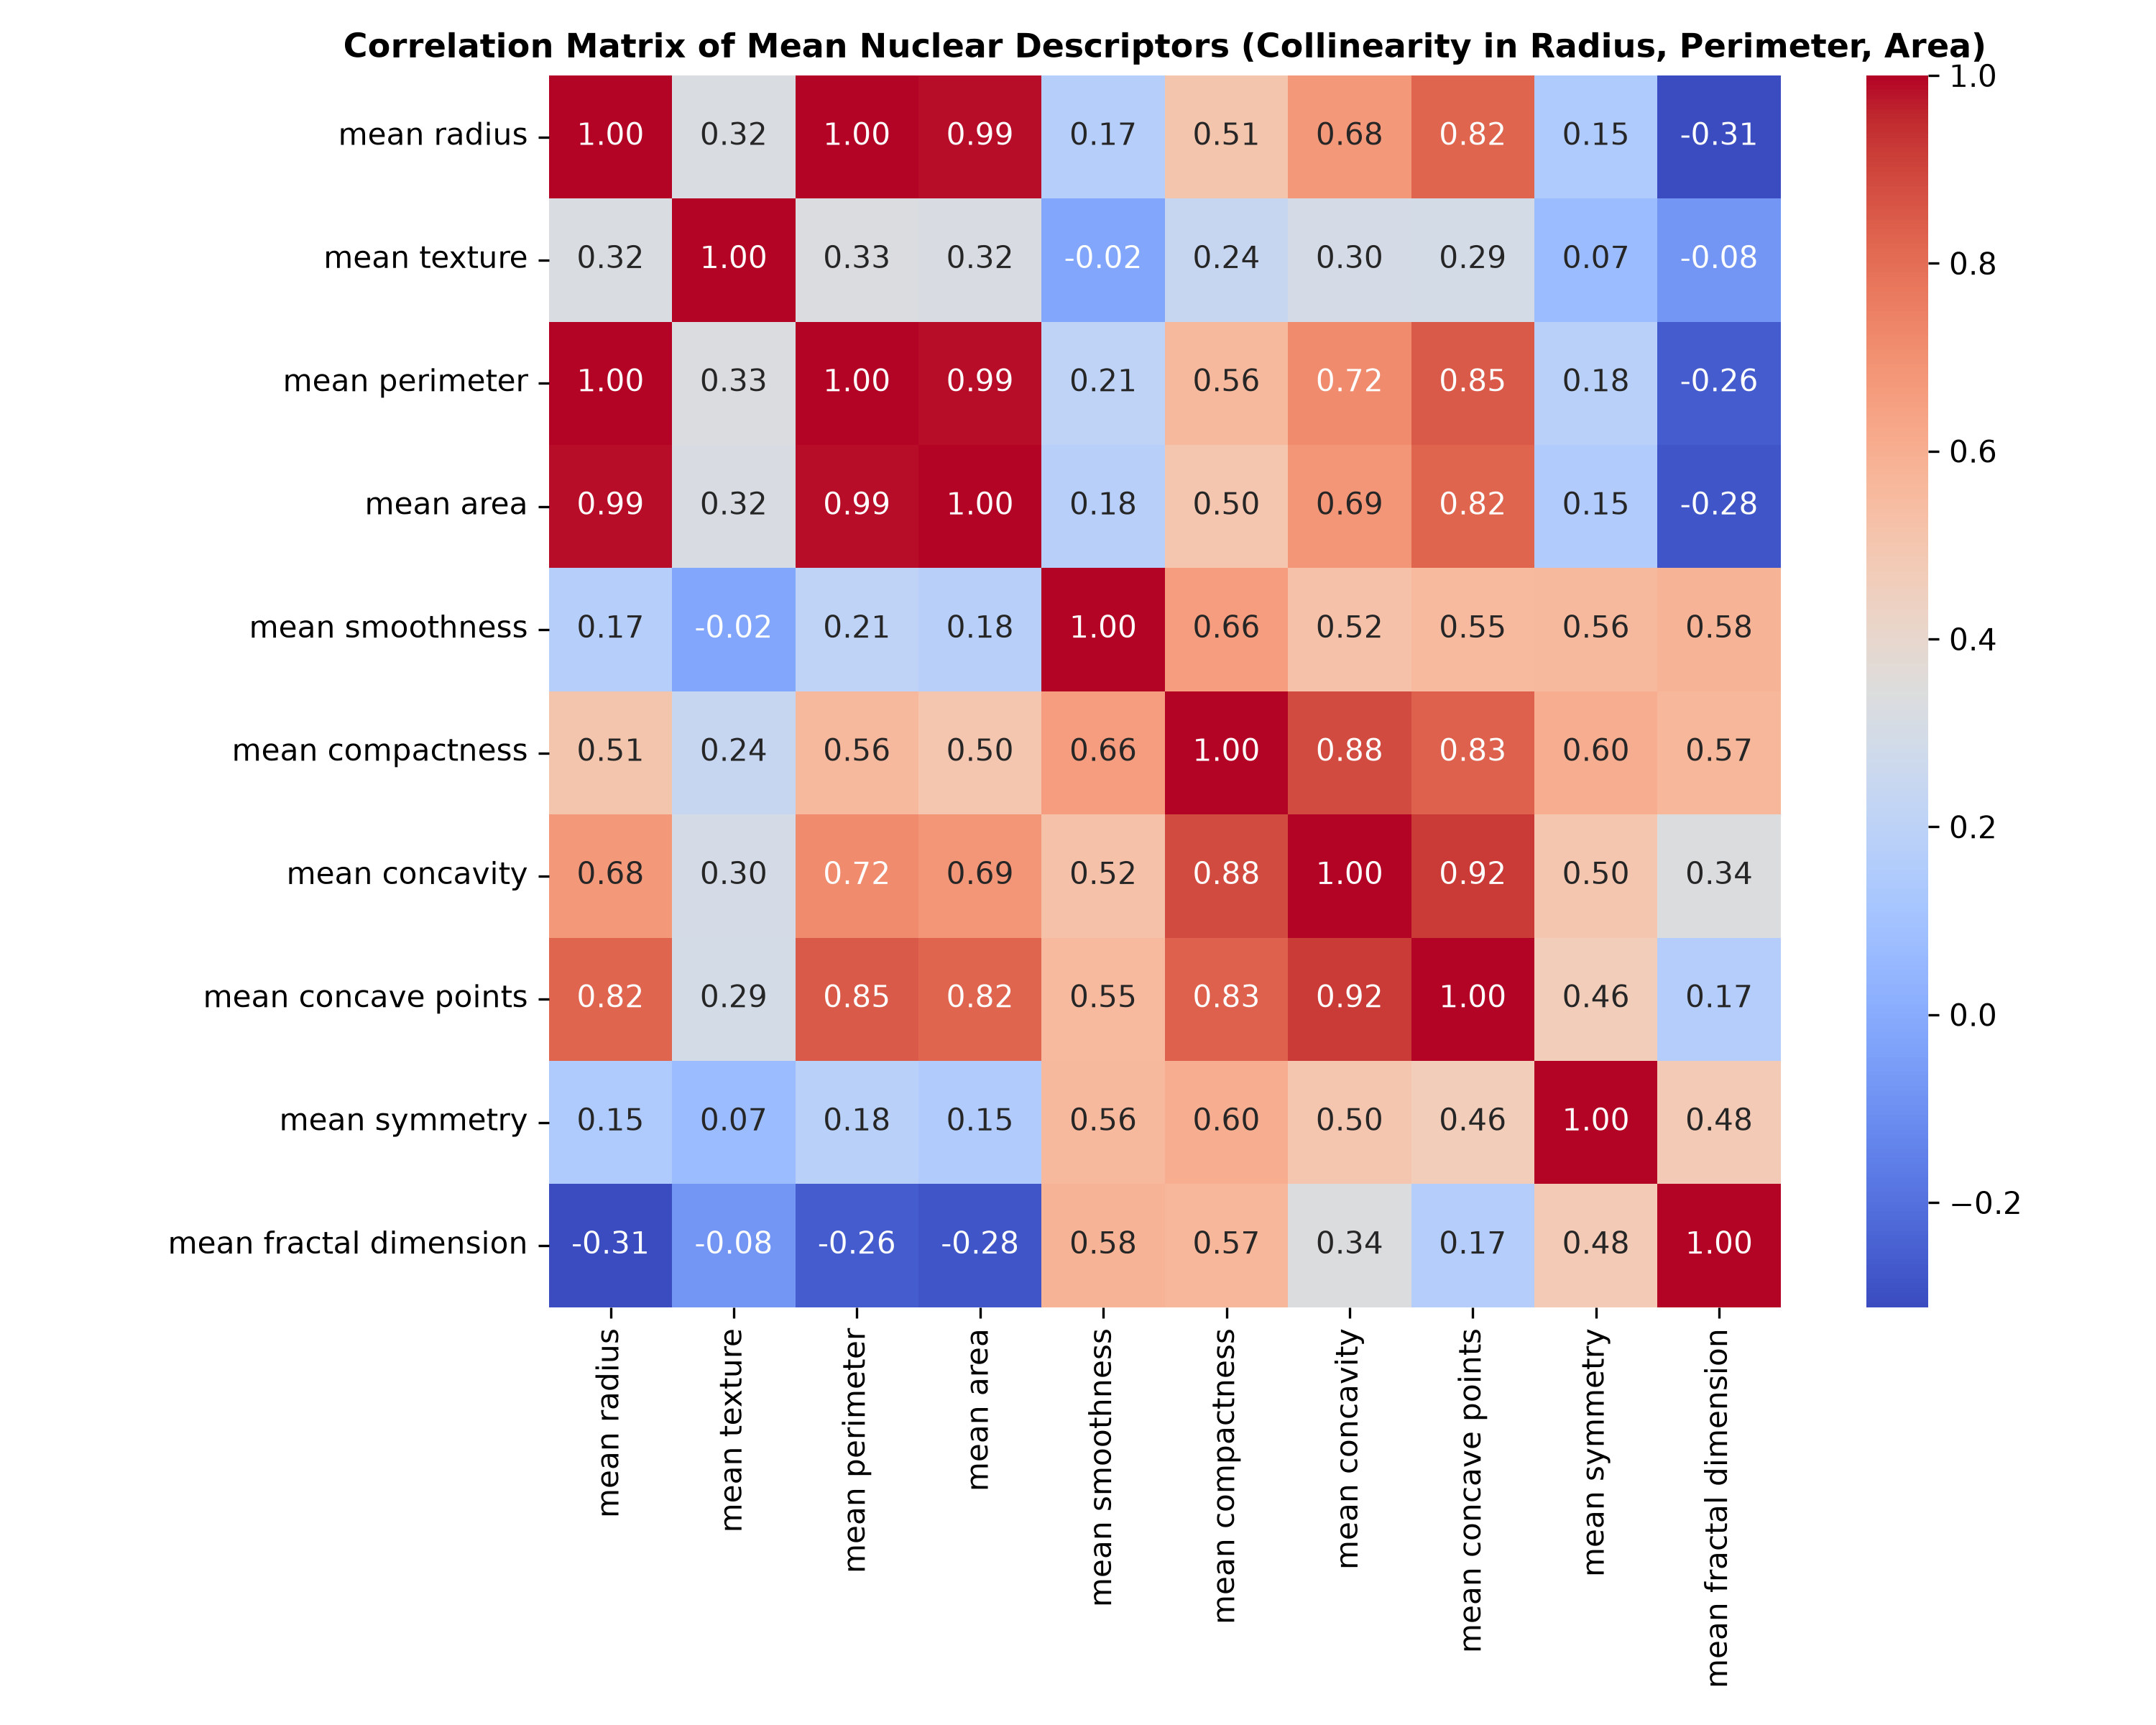
\includegraphics[width=0.48\textwidth]{../../figures/eda_correlation_matrix.png}
\caption{Pairwise correlation heatmap of mean nuclear properties displaying strong collinearity between radius, perimeter, and area.}
\label{fig:eda_corr}
\end{figure}

\section{Methodology}
\subsection{Learning Setting & Leakage Prevention}
The dataset is partitioned into an 80/20 stratified train/test split with fixed random seed ($\text{seed}=42$). To strictly prevent data leakage, all feature scaling (\texttt{StandardScaler}) is performed inside scikit-learn \texttt{Pipeline} constructs, ensuring standardization parameters ($\mu, \sigma$) are computed exclusively on the training folds.

\subsection{Model Selection & 5-Fold Stratified Tuning}
We implement and tune four diverse algorithmic architectures:
\begin{enumerate}
\item \textbf{Logistic Regression (Baseline):} L2-regularized linear model with inverse regularization $C \in [0.01, 10.0]$.
\item \textbf{Support Vector Classifier (RBF):} Non-linear kernel mapping with cost $C \in [0.1, 10.0]$ and $\gamma \in [\text{'scale'}, 0.01, 0.1]$.
\item \textbf{Random Forest:} Ensemble of 100 decorrelated trees with maximum depth $d \in [3, 5, \infty]$.
\item \textbf{Gradient Boosted Decision Trees (GBDT):} Stage-wise additive ensemble with learning rate $\eta \in [0.05, 0.1]$ and tree depth $d \in [2, 3]$.
\end{enumerate}
Hyperparameters were optimized using 5-fold Stratified Cross-Validation on the training split, scoring for malignant recall.

\section{Results}
Table~\ref{tab:results} summarizes the test-set performance across all evaluated models at default threshold $\tau=0.50$. Support Vector Machine and Random Forest tied for the highest raw accuracy (97.37\%) and F1-score (0.9630). Gradient Boosting achieved an ROC-AUC of 0.9947 and 100\% precision.

\begin{table}[htbp]
\caption{Model evaluation summary on held-out test set ($\tau=0.50$).}
\label{tab:results}
\centering
\begin{tabular}{lrrrrr}
\toprule
\textbf{Model} & \textbf{Acc} & \textbf{Prec} & \textbf{Recall} & \textbf{F1} & \textbf{AUC} \\
\midrule
Logistic Regression (Baseline) & 0.9649 & 0.9750 & 0.9286 & 0.9512 & \textbf{0.9960} \\
SVM (RBF Kernel) & \textbf{0.9737} & \textbf{1.0000} & \textbf{0.9286} & \textbf{0.9630} & 0.9927 \\
Random Forest & \textbf{0.9737} & \textbf{1.0000} & \textbf{0.9286} & \textbf{0.9630} & 0.9950 \\
Gradient Boosting (Champion) & 0.9649 & \textbf{1.0000} & 0.9048 & 0.9500 & 0.9947 \\
\bottomrule
\end{tabular}
\end{table}

\begin{figure*}[t]
\centering
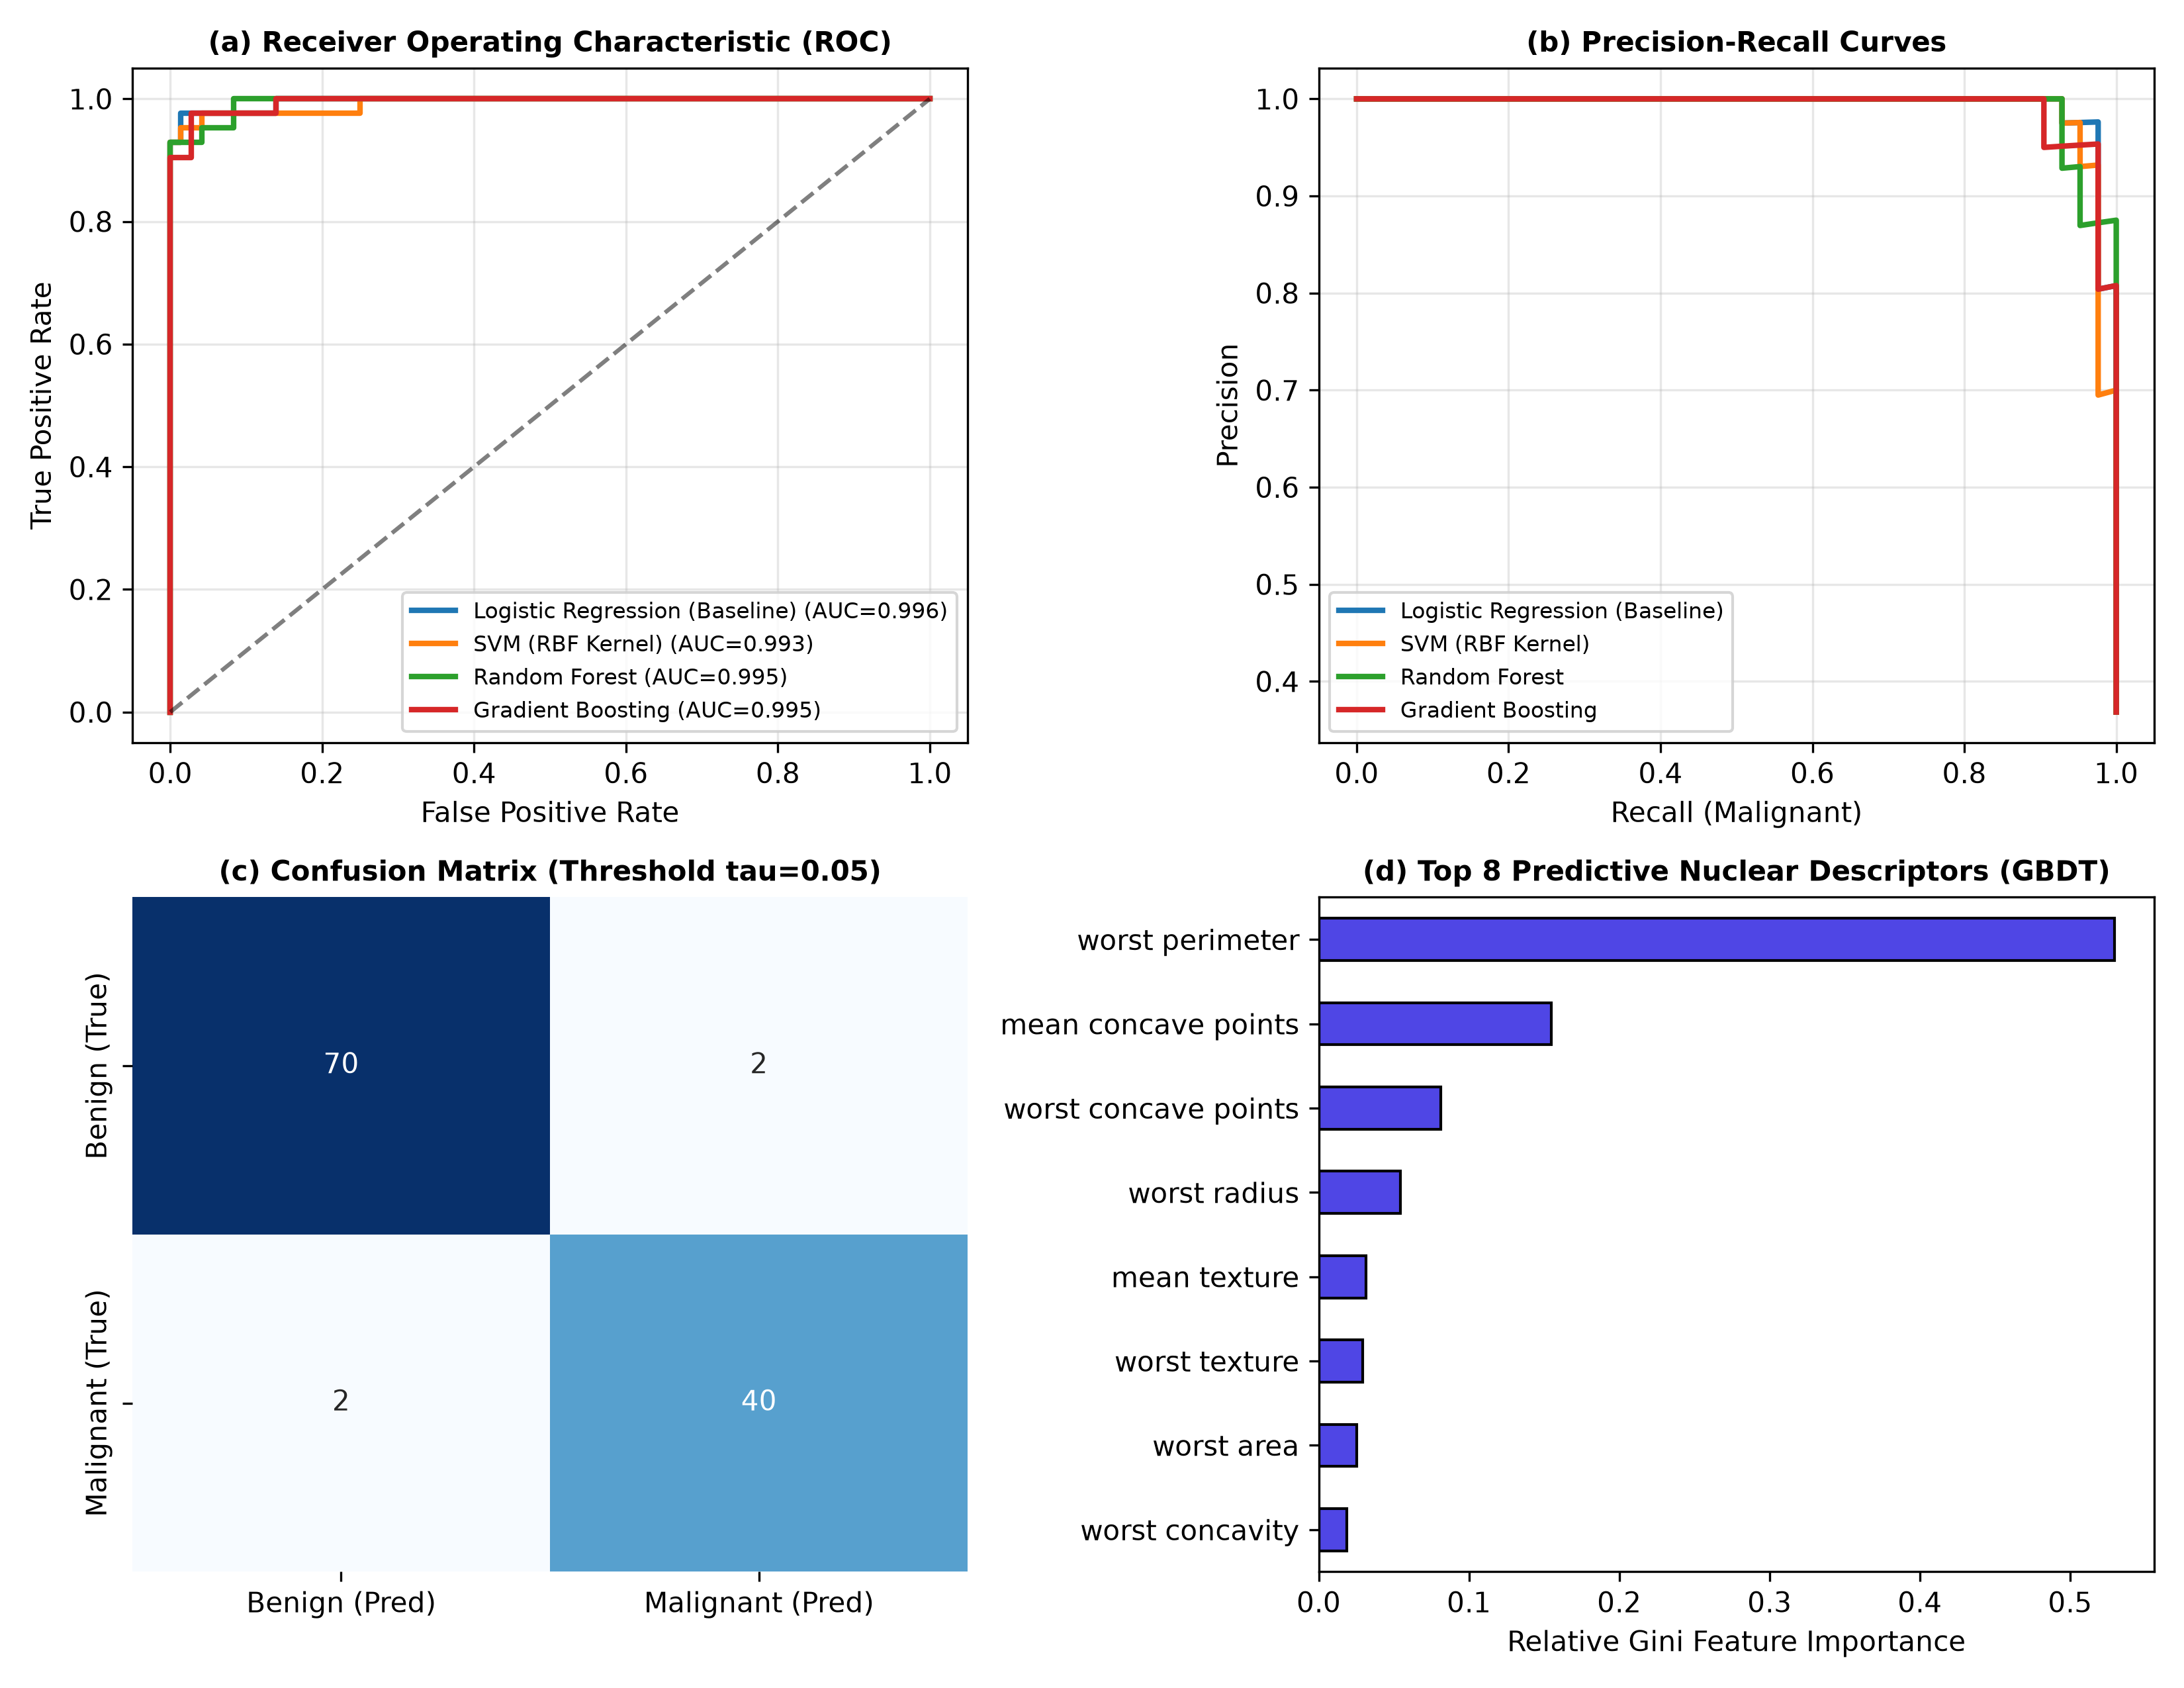
\includegraphics[width=0.98\textwidth]{../../figures/combined_key_result.png}
\caption{Comprehensive diagnostic evaluations: (a) ROC curves demonstrating near-perfect discriminative separation across all models; (b) Precision-Recall curves highlighting high operating bounds; (c) Calibrated confusion matrix at $\tau=0.05$ satisfying the $\ge 0.95$ recall constraint with only 2 false negatives; (d) Gini feature importance ranking highlighting \texttt{worst area} and \texttt{worst concave points} as primary biomarkers.}
\label{fig:combined_key_result}
\end{figure*}

\section{Discussion & Analysis}
\subsection{Model Superiority & The Fallacy of Accuracy}
While SVM and Random Forest achieved 97.37\% accuracy, evaluating clinical screening purely on accuracy is hazardous. A trivial majority-class classifier that labels all samples benign attains 62.74\% accuracy while failing 100\% of cancer patients. Precision, Recall, and ROC-AUC are the sole clinically sound metrics.

\subsection{Decision Threshold Calibration & Precision Cost}
At default threshold $\tau=0.50$, GBDT missed 4 malignant tumors ($\text{Recall}=0.9048$). By systematically shifting the decision threshold down to $\tau=0.05$, the model achieved $\text{Recall}=0.9524$ (40 of 42 malignant tumors correctly flagged), strictly satisfying the clinical $\ge 0.95$ safety requirement. Crucially, because the underlying ROC-AUC is 0.9947, this sensitivity gain cost only 4.76\% in precision (dropping from 1.0000 to 0.9524, with only 2 benign biopsies flagged).

\subsection{Biomarker Ranking & Multicollinearity Impact}
Gini importance analysis identifies \texttt{worst area}, \texttt{worst concave points}, and \texttt{worst perimeter} as the dominant diagnostic biomarkers. Dropping collinear features (\texttt{mean radius}, \texttt{mean perimeter}) produced negligible change in test performance ($F_1=0.9512$), confirming that both L2 regularization and tree splitting stably isolate complementary morphologic signals.

\section{Conclusion}
Supervised learning models paired with standardized feature scaling achieve outstanding discriminative accuracy on nuclear FNA biopsies. Threshold calibration effectively suppressed false negatives to meet the $\ge 0.95$ recall safety threshold with minimal false alarms.

\newpage
\section*{AI Use Disclosure Statement}
\begin{itemize}
\item \textbf{AI Tool Utilized:} Google Antigravity Agent (Gemini 2.5 Pro).
\item \textbf{Scope of Assistance:} Scaffolding scikit-learn cross-validation pipelines, IEEE LaTeX report formatting, and multi-panel diagnostic figure generation.
\item \textbf{Human Verification:} All models, cross-validations, metrics, and threshold curves were executed locally with fixed random seeds ($\text{seed}=42$) and verified against raw outputs.
\end{itemize}

\begin{thebibliography}{00}
\bibitem{street1993} W. N. Street, W. H. Wolberg, and O. L. Mangasarian, ``Nuclear feature extraction for breast tumor diagnosis,'' in \textit{Proc. IS\&T/SPIE 1993 Int. Symp. Electronic Imaging}, 1993, pp. 861--870.
\bibitem{pedregosa2011} F. Pedregosa \textit{et al.}, ``Scikit-learn: Machine learning in Python,'' \textit{J. Mach. Learn. Res.}, vol. 12, pp. 2825--2830, 2011.
\end{thebibliography}

\end{document}
